\documentclass{article}
\usepackage{polski} %moze wymagac dokonfigurowania latexa, ale jest lepszy niż standardowy babel'owy [polish] 
\usepackage[utf8]{inputenc} 
\usepackage[OT4]{fontenc} 
\usepackage{graphicx,color} %include pdf's (and png's for raster graphics... avoid raster graphics!) 
\usepackage{url} 
\usepackage[pdftex,hyperfootnotes=false,pdfborder={0 0 0}]{hyperref} %za wszystkimi pakietami; pdfborder nie wszedzie tak samo zaimplementowane bo specyfikacja nieprecyzyjna; pod miktex'em po prostu nie widac wtedy ramek


% Zmiana rozmiar�w strony tekstu
\addtolength{\voffset}{-1cm}
\addtolength{\hoffset}{-1cm}
\addtolength{\textwidth}{2cm}
\addtolength{\textheight}{2cm}

%bardziej zyciowe parametry sterujace rozmieszczeniem rysunkow
\renewcommand{\topfraction}{.85}
\renewcommand{\bottomfraction}{.7}
\renewcommand{\textfraction}{.15}
\renewcommand{\floatpagefraction}{.66}
\renewcommand{\dbltopfraction}{.66}
\renewcommand{\dblfloatpagefraction}{.66}
\setcounter{topnumber}{9}
\setcounter{bottomnumber}{9}
\setcounter{totalnumber}{20}
\setcounter{dbltopnumber}{9}

% w�asny bullet list z malymi odstepami
\newenvironment{tightlist}{
\begin{itemize}
  \setlength{\itemsep}{1pt}
  \setlength{\parskip}{0pt}
  \setlength{\parsep}{0pt}}
{\end{itemize}}




\begin{document}

\thispagestyle{empty} %bez numeru strony

\begin{center}
{\large{Sprawozdanie II z laboratorium:\\
Uczenie Maszynowe i Sieci Neuronowe}}

\vspace{3ex}

Część I: Uczenie nadzorowane warstwowych sieci neuronowych

Część II: Rekurencyjne sieci neuronowe

Część III: Uczenie nienadzorowane warstwowych sieci neuronowych


\vspace{3ex}
{\footnotesize\today}

\end{center}


\vspace{10ex}

Prowadzący: dr inż. Maciej Komosiński

\vspace{5ex}

Autorzy:
\begin{tabular}{lllr}
\textbf{Krzysztof Urban} & inf84896 & ISWD & krz.urb@gmail.com \\
\textbf{Tomasz Ziętkiewicz} & inf84914 & ISWD & tomek.zietkiewicz@gmail.com \\
\end{tabular}

\vspace{5ex}

Zajęcia poniedziałkowe; Krzysztof: 16:50, Tomasz: 13:30

\newpage



%%%%%%%%%%%%%%%%%% Część I %%%%%%%%%%%%%%%%%

\section{Generowanie drzew decyzyjnych}

\subsection{Generowanie drzewa}

\begin{itemize}
\item \textbf{Obejrzyj zawartość plików \emph{golf.nam}, \emph{golf.dat} i~\emph{golf.tst}; ile przykładów zawiera zbiór uczący? Iloma atrybutami są~one opisane?}
	\\Zbiór uczący zawiera 14 przykładów. Są one opisane pięcioma atrybutami, w tym jednym atrybutem decyzyjnym.

\item \textbf{Wygeneruj drzewo dla zbioru przykładów \emph{golf}; ustawienia standardowe.}
	\begin{center}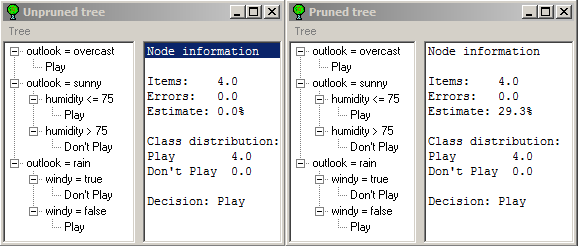
\includegraphics[width=1\textwidth]{drzewo.png}\end{center}

\item \textbf{Przeanalizuj wyniki; czy udało się przeprowadzić pruning?}
	\\Nie udało się przeprowadzić pruningu. Drzewa są identyczne.

\item \textbf{Obejrzyj drzewo; ile ma węzłów decyzyjnych, a~ile liści?}
	\\Wygenerowane drzewo ma 3 węzły decyzyjne i 5 liści.

\item \textbf{ Prześledź ścieżkę od korzenia do wybranego liścia.
}		\\Korzeń jest węzłem związanym z atrybutem outlook. Jeśli dla klasyfikowanego przykładu wartość atrybutu outlook wynosi "sunny", to następny węzeł na ścieżce to ten związany z atrybutem humidity. Zakłądając, że dla naszego przykładu wilgotność jest większ niż $ 75\% $ , liściem w analizowanej ścieżce będzie liść odnoszący się decyzji "Don't Play".
		\\Inaczej mówiąc, ścieżk ta klasyfikuje wszystkie dni w które jest słoneczna pogoda i wilgotność większa niż $ 75\% $ jako dni, w które nie gra się w golfa.
		
\item \textbf{Porównaj estymaty błędu dla drzewa oryginalnego (\emph{Unpruned}) i~uproszczonego (\emph{Pruned}).}
	\\Estymata błędu dla oryginalnego drzewa wynosi  $ 0\% $ a dla uproszczonego $ 38,5\% $ .

\item \textbf{Obejrzyj macierz pomyłek.}
	\\Ponieważ drzewo oryginalne nie generuje błędów dla zbioru uczącego to też jedyne co możemy z niego odczytać, to właśnie, że żadne obiekty nie są błędnie klasyfikowane, oraz że w przypadku 9 przykładów drzewo poprawnie zaklasyfikowało przykłądy do klasy "Play" a w 5 przypadkach do klasy "Don't Play".

\end{itemize}

\subsection{Konsultowanie}

\begin{itemize}
\item Dokonaj konsultacji wymyślonego przykładu dla wygenerowanego drzewa.
\item Konsultowanie przykładu ,,niepełnego''; dokładnie przeanalizuj wynik.
\item Konsultowanie, gdy znany jest rozkład prawdopodobieństwa.
\end{itemize}

\subsection{Różnica między \emph{gain ratio} a~\emph{info gain} w~praktyce}

\begin{itemize}
\item Obejrzyj zbiór \emph{testgain} (\emph{dat} i~\emph{nam}).
\item Wygeneruj dla niego dwukrotnie drzewo z~użyciem opcji \emph{gain ratio} i~\emph{info gain}; skomentuj wyniki.
\end{itemize}

\subsection{Grupowanie wartości atrybutów}

\begin{itemize}
\item Wygeneruj drzewo dla zbioru \emph{testgain}, zaznaczając opcję \emph{Subsetting}.
\item Analogicznie dla \emph{CRX}: opisać problem (przyznawanie kard kretytowych), obejrzeć zbiór (atrybuty \emph{A4}, \emph{A6} i~\emph{A7} mają wiele wartości); wygenerować drzewo bez i~z~grupowaniem.
\item Obejrzeć macierz pomyłek dla zbioru uczącego i~testującego; czy w~tym zastosowaniu przydałaby się macierz kosztów pomyłek?
\end{itemize}

\subsection{Poszukiwanie optymalnej wielkości drzewa uproszczonego}

\begin{itemize}
\item Poszukiwanie optymalnej wielkości drzewa uproszczonego przez dobór poziomu ufności procedury upraszczającej (\emph{Pruning confidence level}); przeprowadź serię eksperymentów \emph{10-fold cross-validation} dla zbioru \emph{Monk2}, ze~zmieniającym się poziomem ufności od~0.05 do~0.5, z~krokiem co najwyżej 0.05. Sporządź wykres zależności:

\begin{itemize}
\item średniego (po \emph{cross-validation}) rozmiaru drzewa uproszczonego,
\item średniej trafności klasyfikowania drzewa uproszczonego na~zbiorze testującym,
\item średniej estymaty błędu dla drzewa uproszczonego
\end{itemize}

...w funkcji poziomu ufności (odnieś te wyniki do średniej charakterystyki drzewa oryginalnego, nieuproszczonego).

\item Poszukiwanie optymalnej wielkości drzewa uproszczonego poprzez prepruning, tj.~manewrowanie minimalną licznością węzła (\emph{Minimum objects}). Dla zbioru \emph{CRX} przebadać przedział od~2 do~10.
\item Analiza wygenerowanego drzewa: poszukiwanie słabych punktów (liści o~małym wsparciu, poddrzew które generują szczególnie dużo błędów, etc.).
\end{itemize}

\subsection{\emph{Windowing}}

\begin{itemize}
\item Wyjaśnić zasadę i~opcje: \emph{Trials}, \emph{Initial window size}, \emph{Window increment}.
\item Analiza wyników (\emph{CRX}).
\end{itemize}

\subsection{Generowanie krzywej uczenia}

\begin{itemize}
\item Dla zbioru \emph{vote} przygotować kilka[naście] zbiorów uczących o~liczności $n$ zmieniającej się od~50 do~300, ze~skokiem np.~50 przypadków, poprzez wybieranie pierwszych $n$ ze~zbioru \emph{vote.dat}.
\item Wykreślić jako funkcję $n$ rozmiar drzewa uproszczonego oraz trafność klasyfikowania drzewa uproszczonego na zbiorze testującym.

\end{itemize}

\subsection{Maksymalizacja trafności}

\begin{itemize}
\item Uzyskaj jak najwyższą trafność klasyfikowania ze~zbioru \emph{GERMAN} w~eksperymencie \emph{10-fold CV}. Jakimi parametrami i~mechanizmami można manipulować, by~szukać najwyższej trafności? Kiedy można ufać tak uzyskanej trafności, a~kiedy można mówić o~nadużyciu?
\end{itemize}

%%%%%%%%%%%%%%%%%% Część II %%%%%%%%%%%%%%%%%

\section{Generowanie reguł decyzyjnych}

\subsection{Metoda pośrednia generowania reguł (\emph{C4.5rules})}

\begin{itemize}
\item Wygeneruj reguły dla zbioru \emph{GOLF} za~pomocą programu \emph{C4.5 for Windows}.
\item Porównaj wygenerowane reguły z~wyjściowym drzewem decyzyjnym. Czy reguły odzwierciedlają precyzyjnie drzewo?
\end{itemize}

\subsection{Porównanie klasyfikowania za pomocą drzew decyzyjnych i~reguł decyzyjnych (\emph{C4.5rules})}

\begin{itemize}
\item Przeprowadź testy \emph{10-fold CV} na wybranych zbiorach dla drzew i~reguł.
\item Porównaj wyniki pod kątem trafności klasyfikowania na zbiorze testującym oraz rozmiaru opisu.
\item Przeprowadzając kilka eksperymentów uczenia i~testowania przeanalizuj wpływ parametrów \emph{Confidence Level} i~\emph{Redundancy Factor} na~otrzymywany zbiór reguł.
\end{itemize}

\subsection{Generowanie reguł z~użyciem algorytmu \emph{LEM}}

\begin{itemize}
\item Wygeneruj reguły dla zbioru \emph{HPAP.ISF}.
\item Przyjrzyj się regułom możliwym; opisz je i~,,wydedukuj'', skąd się wzięły.
\end{itemize}

\subsection{Porównanie reguł generowanych za~pomocą algorytmu \emph{LEM} i~\emph{C4.5}}

\begin{itemize}
\item Wygeneruj reguły przy użyciu obu podejść dla zbiorów: \emph{HPAP}, \emph{VOTE} i~\emph{MONK}.
\item Przyjrzyj się niezależnie regułom pewnym i~możliwym (\emph{LEM}).
\end{itemize}

%Dla chętnych:
%\subsection{Przeprowadź eksperyment generowania i~testowania reguł LEM w~ramach cross validation}

%%%%%%%%%%%%%%%% literatura %%%%%%%%%%%%%%%%

\bibliography{sprawozd}
\bibliographystyle{plain}


\end{document}

